\documentclass[xcolor=dvipsnames]{beamer}
\makeatletter\def\Hy@xspace@end{}\makeatother 
\usepackage{graphicx, color, amssymb, amsmath, bm, rotating, graphics,
epsfig, multicol, amsthm, animate}
\usepackage{media9}
\usepackage[english]{babel}
\usepackage[T1]{fontenc}
\usepackage[ansinew]{inputenc}
\usepackage[authoryear]{natbib}
%\newcommand{\newblock}{}  %needed to make beamer and natbib play nice
\usepackage{tikz, caption}
% A counter, since TikZ is not clever enough (yet) to handle
% arbitrary angle systems.
\newcount\mycount

\usetheme{Boadilla}
%\usecolortheme{lily}
\definecolor{MUgold}{RGB}{241,184,45}
\usecolortheme[named=MUgold]{structure}
\setbeamercolor{structure}{bg=Black}
\setbeamercolor{structure}{fg=MUgold}
\setbeamercolor{title}{bg=Black}
\setbeamercolor{frametitle}{bg=Black, fg=MUgold}
\setbeamercolor{title in head/foot}{fg=Black, bg=MUgold}
\setbeamercolor{author in head/foot}{fg=MUgold, bg=Black}
\setbeamercolor{institute in head/foot}{fg=MUgold, bg=Black}
\setbeamercolor{date in head/foot}{fg=MUgold, bg=Black}
\setbeamercolor{item projected}{bg=MUgold, fg=Black}
\usesubitemizeitemtemplate{\tiny\raise1.5pt\hbox{\color{Black}$\blacktriangleright$}}
\setbeamercovered{transparent=0}
\beamertemplatenavigationsymbolsempty

\title[AT-PSO for Spatial Design]{Adaptively Tuned Particle Swarm Optimization for Spatial Design}

%\subtitle{}
\author[Matt Simpson]{Matthew Simpson}
\institute[Mizzou Stat / SAS]{Department of Statistics, University of Missouri\\
                              SAS Institute, Inc.}
\date{August 3, 2016}

\begin{document}

\begin{frame}
\titlepage
\centering
{\scriptsize
Joint work with Christopher Wikle and Scott H. Holan\\~\\
Research supported by the NSF-Census Research Network}
\end{frame}

\begin{frame}
\frametitle{Overview of the Talk}
\begin{columns}
\begin{column}{0.5\textwidth}
\begin{enumerate}
\item What is particle swarm optimization (PSO)?\\
 \citep{blum2008swarm, clerc2010particle, clerc2011spso}\\~\\
\item New adaptively-tuned PSO algorithms.\\~\\
\item Using (adaptively-tuned) PSO for spatial design.\\~\\
\item Example adding to an existing monitoring network.
\end{enumerate}
\end{column}
\begin{column}{0.5\textwidth}
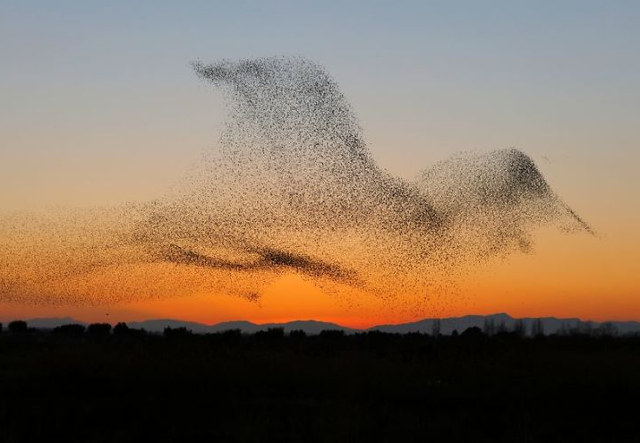
\includegraphics[width = 0.99\textwidth]{birds3.jpg}
\end{column}
\end{columns}
\end{frame}

\begin{frame}
\frametitle{Particle Swarm Optimization --- Intuition}
\begin{center}
\includemedia[
  width=0.9\textwidth,
  activate=pagevisible,
  deactivate=pageinvisible,
  addresource=fishschool.mp4,   %passcontext,  %show VPlayer's right-click menu
  flashvars={
    %important: same path as in `addresource'
    source=fishschool.mp4
    &autoPlay=true
    &loop=true
  }
]{\fbox{Click!}}{VPlayer.swf}
\end{center}
Put a ``swarm'' of particles in the search space:\\
\begin{itemize}
\item[] Don't search alone, pay attention to what your neighbors are doing!
\end{itemize}
\end{frame}

\begin{frame}
\frametitle{Particle Swarm Optimization}
Goal: minimize some objective function $Q(\bm{\theta}): \mathbb{R}^D \to \mathbb{R}$.\\~\\
Populate $\Theta$ with $n$ particles. Define particle $i$ in period $k$ by:
\begin{itemize}
\item a {\color{red}location} \hfill $\bm{\theta}_i(k)\in \mathbb{R}^D$;\hspace{2.5cm}\phantom{.}
\item a {\color{red}velocity} \hfill $\bm{v}_i(k) \in \mathbb{R}^D$;\hspace{2.5cm}\phantom{.}
\item a {\color{red}personal best} location \hfill $\bm{p}_i(k) \in \mathbb{R}^D$;\hspace{2.5cm}\phantom{.} 
\item a {\color{red}neighborhood (group) best} location \hfill $\bm{g}_i(k) \in \mathbb{R}^D$.\hspace{2.5cm}\phantom{.} \\~\\
\end{itemize}

\pause 

Basic PSO: update particle $i$ from $k$ to $k+1$ via: \\
\begin{itemize}
\item  For $j=1,2,\dots,D$:
\begin{align*}
v_{ij}(k+1) &= {\color{blue}\omega} v_{ij}(k) +  \mathrm{U}(0,{\color{blue}\phi_1})\times\{p_{ij}(k) - \theta_{ij}(k)\} \\
     &\;\phantom{= \omega v_{ij}(k)}+  \mathrm{U}(0,{\color{blue}\phi_2})\times\{g_{ij}(k) - \theta_{ij}(k)\}\\
& = \mbox{{\color{red}inertia}} + \mbox{{\color{red}cognitive}} + \mbox{{\color{red}social}},\\
\theta_{ij}(k+1) &= \theta_{ij}(k) + v_{ij}(k+1),
\end{align*}
\item Then update personal and group best locations.
\end{itemize}
\end{frame}

\begin{frame}
\frametitle{PSO --- Parameters}
{\color{red}Inertia} parameter: $\omega$.
\begin{itemize}
\item Controls the particle's tendency to keep moving in the same direction.\\~\\
\end{itemize}

{\color{red}Cognitive} correction factor: $\phi_1$.
\begin{itemize}
\item Controls the particle's tendency to move toward its personal best.\\~\\
\end{itemize}

{\color{red}Social} correction factor: $\phi_2$.
\begin{itemize}
\item Controls the particle's tendency to move toward its neighborhood best.\\~\\
\end{itemize}

Default choices:
\begin{itemize}
\item $\omega = 0.7298$, $\phi_1 = \phi_2 = 1.496$ \citep{clerc2002particle}.
\item $\omega = 1/(2\ln 2)\approx 0.721$, $\phi_1=\phi_2=1/2 + \ln 2\approx 1.193$ \citep{clerc2006stagnation}.
\end{itemize}

\end{frame}

\begin{frame}
\frametitle{PSO --- Neighborhood Topologies}
Sometimes it is useful to restrict the flow of information across the swarm --- e.g. complicated objective functions with many local optima.\\~\\

Particles are only informed by their \emph{neighbors}. \\~\\

\pause

Easy to visualize example: Ring-$k$ neighborhood topology.
\begin{figure}
  \centering
  {
    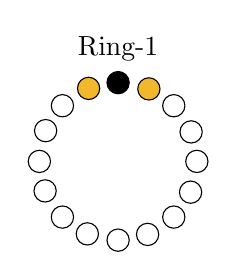
\begin{tikzpicture}[transform shape]
      % the multiplication with floats is not possible. Thus I split the loop in two.
      \foreach \number in {1,...,2}{
        % Computer angle:
        \mycount=\number
        \advance\mycount by 0
        \multiply\mycount by 45
        \advance\mycount by 22.5
        \node[circle,inner sep=0.1cm,fill=MUgold] (N-\number) at (\the\mycount:1cm) {};
      }
      \foreach \number in {1,...,1}{
        % Computer angle:
        \mycount=\number
        \advance\mycount by 1
        \multiply\mycount by 45
        \advance\mycount by 0
        \node[draw=black,circle,inner sep=0.1cm,fill=black,label=Ring-1] (N-\number) at (\the\mycount:1cm) {};
        \foreach \number in {1,...,7}{
          % Computer angle:
          \mycount=\number
          \advance\mycount by 2
          \multiply\mycount by 45
          \advance\mycount by 0
          \node[draw,circle,inner sep=0.1cm] (N-\number) at (\the\mycount:1cm) {};
        }
        \foreach \number in {8,...,15}{
          % Computer angle:
          \mycount=\number
          \advance\mycount by 1
          \multiply\mycount by 45
          \advance\mycount by 22.5
          \node[draw,circle,inner sep=0.1cm] (N-\number) at (\the\mycount:1cm) {};
        }
      }
    \end{tikzpicture}
  }
  {
    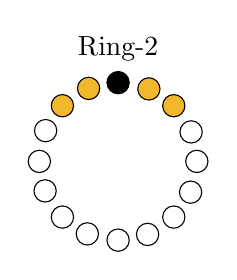
\begin{tikzpicture}[transform shape]
      % the multiplication with floats is not possible. Thus I split the loop in two.
      \foreach \number in {1,...,2}{
        % Computer angle:
        \mycount=\number
        \advance\mycount by 0
        \multiply\mycount by 45
        \advance\mycount by 22.5
        \node[circle,inner sep=0.1cm,fill=MUgold] (N-\number) at (\the\mycount:1cm) {};
      }
      \foreach \number in {1,...,3}{
        % Computer angle:
        \mycount=\number
        \advance\mycount by 0
        \multiply\mycount by 45
        \advance\mycount by 0
        \node[circle,inner sep=0.1cm,fill=MUgold] (N-\number) at (\the\mycount:1cm) {};
      }
      \foreach \number in {1,...,1}{
        % Computer angle:
        \mycount=\number
        \advance\mycount by 1
        \multiply\mycount by 45
        \advance\mycount by 0
        \node[draw=black,circle,inner sep=0.1cm,fill=black,label=Ring-2] (N-\number) at (\the\mycount:1cm) {};
        \foreach \number in {1,...,7}{
          % Computer angle:
          \mycount=\number
          \advance\mycount by 2
          \multiply\mycount by 45
          \advance\mycount by 0
          \node[draw,circle,inner sep=0.1cm] (N-\number) at (\the\mycount:1cm) {};
        }
        \foreach \number in {8,...,15}{
          % Computer angle:
          \mycount=\number
          \advance\mycount by 1
          \multiply\mycount by 45
          \advance\mycount by 22.5
          \node[draw,circle,inner sep=0.1cm] (N-\number) at (\the\mycount:1cm) {};
        }
      }
    \end{tikzpicture}
  }
  {
    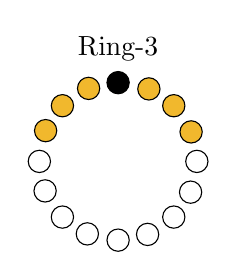
\begin{tikzpicture}[transform shape]
      % the multiplication with floats is not possible. Thus I split the loop in two.
      \foreach \number in {1,...,4}{
        % Computer angle:
        \mycount=\number
        \advance\mycount by -1
        \multiply\mycount by 45
        \advance\mycount by 22.5
        \node[circle,inner sep=0.1cm,fill=MUgold] (N-\number) at (\the\mycount:1cm) {};
      }
      \foreach \number in {1,...,3}{
        % Computer angle:
        \mycount=\number
        \advance\mycount by 0
        \multiply\mycount by 45
        \advance\mycount by 0
        \node[circle,inner sep=0.1cm,fill=MUgold] (N-\number) at (\the\mycount:1cm) {};
      }
      \foreach \number in {1,...,1}{
        % Computer angle:
        \mycount=\number
        \advance\mycount by 1
        \multiply\mycount by 45
        \advance\mycount by 0
        \node[draw=black,circle,inner sep=0.1cm,fill=black,label=Ring-3] (N-\number) at (\the\mycount:1cm) {};
        \foreach \number in {1,...,7}{
          % Computer angle:
          \mycount=\number
          \advance\mycount by 2
          \multiply\mycount by 45
          \advance\mycount by 0
          \node[draw,circle,inner sep=0.1cm] (N-\number) at (\the\mycount:1cm) {};
        }
        \foreach \number in {8,...,15}{
          % Computer angle:
          \mycount=\number
          \advance\mycount by 1
          \multiply\mycount by 45
          \advance\mycount by 22.5
          \node[draw,circle,inner sep=0.1cm] (N-\number) at (\the\mycount:1cm) {};
        }
      }
    \end{tikzpicture}
  }
  {
    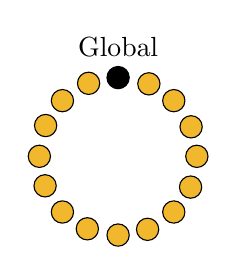
\begin{tikzpicture}[transform shape]
      % the multiplication with floats is not possible. Thus I split the loop in two.
      \foreach \number in {2,...,8}{
        % Computer angle:
        \mycount=\number
        \advance\mycount by 1
        \multiply\mycount by 45
        \advance\mycount by 0
        \node[draw,circle,inner sep=0.1cm,fill=MUgold] (N-\number) at (\the\mycount:1cm) {};
      }
      \foreach \number in {9,...,16}{
        % Computer angle:
        \mycount=\number
        \advance\mycount by 1
        \multiply\mycount by 45
        \advance\mycount by 22.5
        \node[draw,circle,inner sep=0.1cm,fill=MUgold] (N-\number) at (\the\mycount:1cm) {};
      }
      \foreach \number in {1,...,1}{
        % Computer angle:
        \mycount=\number
        \advance\mycount by 1
        \multiply\mycount by 45
        \advance\mycount by 0
        \node[draw=black,circle,inner sep=0.1cm,fill=black,label=Global] (N-\number) at (\the\mycount:1cm) {};
      }
    \end{tikzpicture}
  }
\end{figure}
Each particle is informed by $k$ neighbors to the left and $k$ to the right,\\
\emph{\ \ \ no matter where they are in the search space}.
\end{frame}

\begin{frame}
\frametitle{Stochastic Star Topology, and Other Bells and Whistles}
We use the stochastic star neighborhood topology \citep{miranda2008stochastic}.
\begin{itemize}
\item Each particle informs itself and $m$ random particles.\\
$\to$ sampled with replacement once during initialization.
\item On average each particle is informed by $m$ particles.
\item A small number of particles will be informed by many particles.\\~\\
\end{itemize}

\pause

Many variants available \citep{clerc2011spso}, \citep[][appendix]{simpson2017adaptively}.
\begin{itemize}
\item Handling search space constraints.
\item Coordinate free velocity updates.
\item Parallelization.
\item Asynchronous updates.
\item Redraw neighborhoods.
\end{itemize}
\end{frame}

\begin{frame}
\frametitle{Bare Bones PSO (BBPSO)}
Developed by \citet{kennedy2003bare}.\\~\\

Strips out the velocity term:
\begin{align*}
\theta_{ij}(k+1) \sim \mathrm{N}\left(\frac{p_{ij}(k) + g_{ij}(k)}{2}, |p_{ij}(k) - g_{ij}(k)|^2\right).
\end{align*}
Mimics the behavior of standard PSO.\\~\\

Easier to analyze, but tends to perform worse.
\end{frame}

\begin{frame}
\frametitle{Adaptively Tuned BBPSO}
Add flexibility to the scale parameter:
\begin{align*}
\theta_{ij}(k+1) \sim \mathrm{T}_{df}\left(\frac{p_{ij}(k) + g_{ij}(k)}{2}, \sigma^2(k)|p_{ij}(k) - g_{ij}(k)|^2\right).
\end{align*}
with e.g. $df = 1$ by default.
\begin{itemize}
\item Larger $\sigma^2(k)$: more exploration.
\item Smaller $\sigma^2(k)$: more exploitation.\\~\\
\end{itemize}
How to choose $\sigma^2(k)$'s progression? \\~\\

\pause 

Analogy with adaptively tuned random walk Metropolis.\\
\ \  \citep{andrieu2008tutorial}
\end{frame}

\begin{frame}
\frametitle{Adaptively Tuned BBPSO --- $\sigma^2(k)$'s progression}
Define the improvement rate of the swarm in period $k$:
\begin{align*}
R(k) = &&  \mbox{proportion of particles that improved}\\
       &&  \mbox{on their personal best last period.}
\end{align*}
\pause
Let ${\color{blue}R^*}$ denote a target improvement rate, and\\
\ \ ${\color{blue}c}$ denote an adjustment factor.\\~

Update $\sigma^2(k)$ via:
\begin{align*}
\log \sigma^2(k+1) &= \log\sigma^2(k) + {\color{blue}c}\{R(k+1) - {\color{blue}R^*}\}
\end{align*}
\pause
Larger $c$, faster changes to $\sigma^2(k)$.\\~

\pause

Defaults: $R^*\in[0.3, 0.5]$, $c = 0.1$.
\end{frame}

\begin{frame}
\frametitle{Adaptively Tuning PSO}
In PSO larger $\omega$ $\implies$ more exploration, smaller $\omega$ $\implies$ more exploitation.\\~\\

\pause

Idea: deterministic inertia PSO (DI-PSO) \\
\ \ \ \ \ \ \ $\to$ slowly decrease $\omega(k)$ over time \citep{eberhart2000comparing}.
\begin{itemize}
\item Hard to set appropriately for any given problem.\\~\\
\end{itemize}

\pause

 AT-PSO: tune $\omega(k)$ just like $\sigma^2(k)$ in AT-BBPSO.
\begin{align*}
\log\omega(k+1) = \log\omega(k) + c\{R(k+1) - R^*\}.
\end{align*}
\pause
Same defaults: $R^*\in[0.3, 0.5]$, $c = 0.1$.\\~\\

\pause

Similar PSO algorithm in spirit: \cite{zhang2003adaptive}.
\begin{itemize} 
\item $\omega$ is constant while $\phi_1$ and $\phi_2$ vary across time {\color{red}\emph{and particle}}. 
\item Can't use the same method to adapt $\phi_1$ and $\phi_2$.
\end{itemize}
\end{frame}

\begin{frame}
Example progressions of $\sigma^2(k)$ (left) and $\omega(k)$ (right):
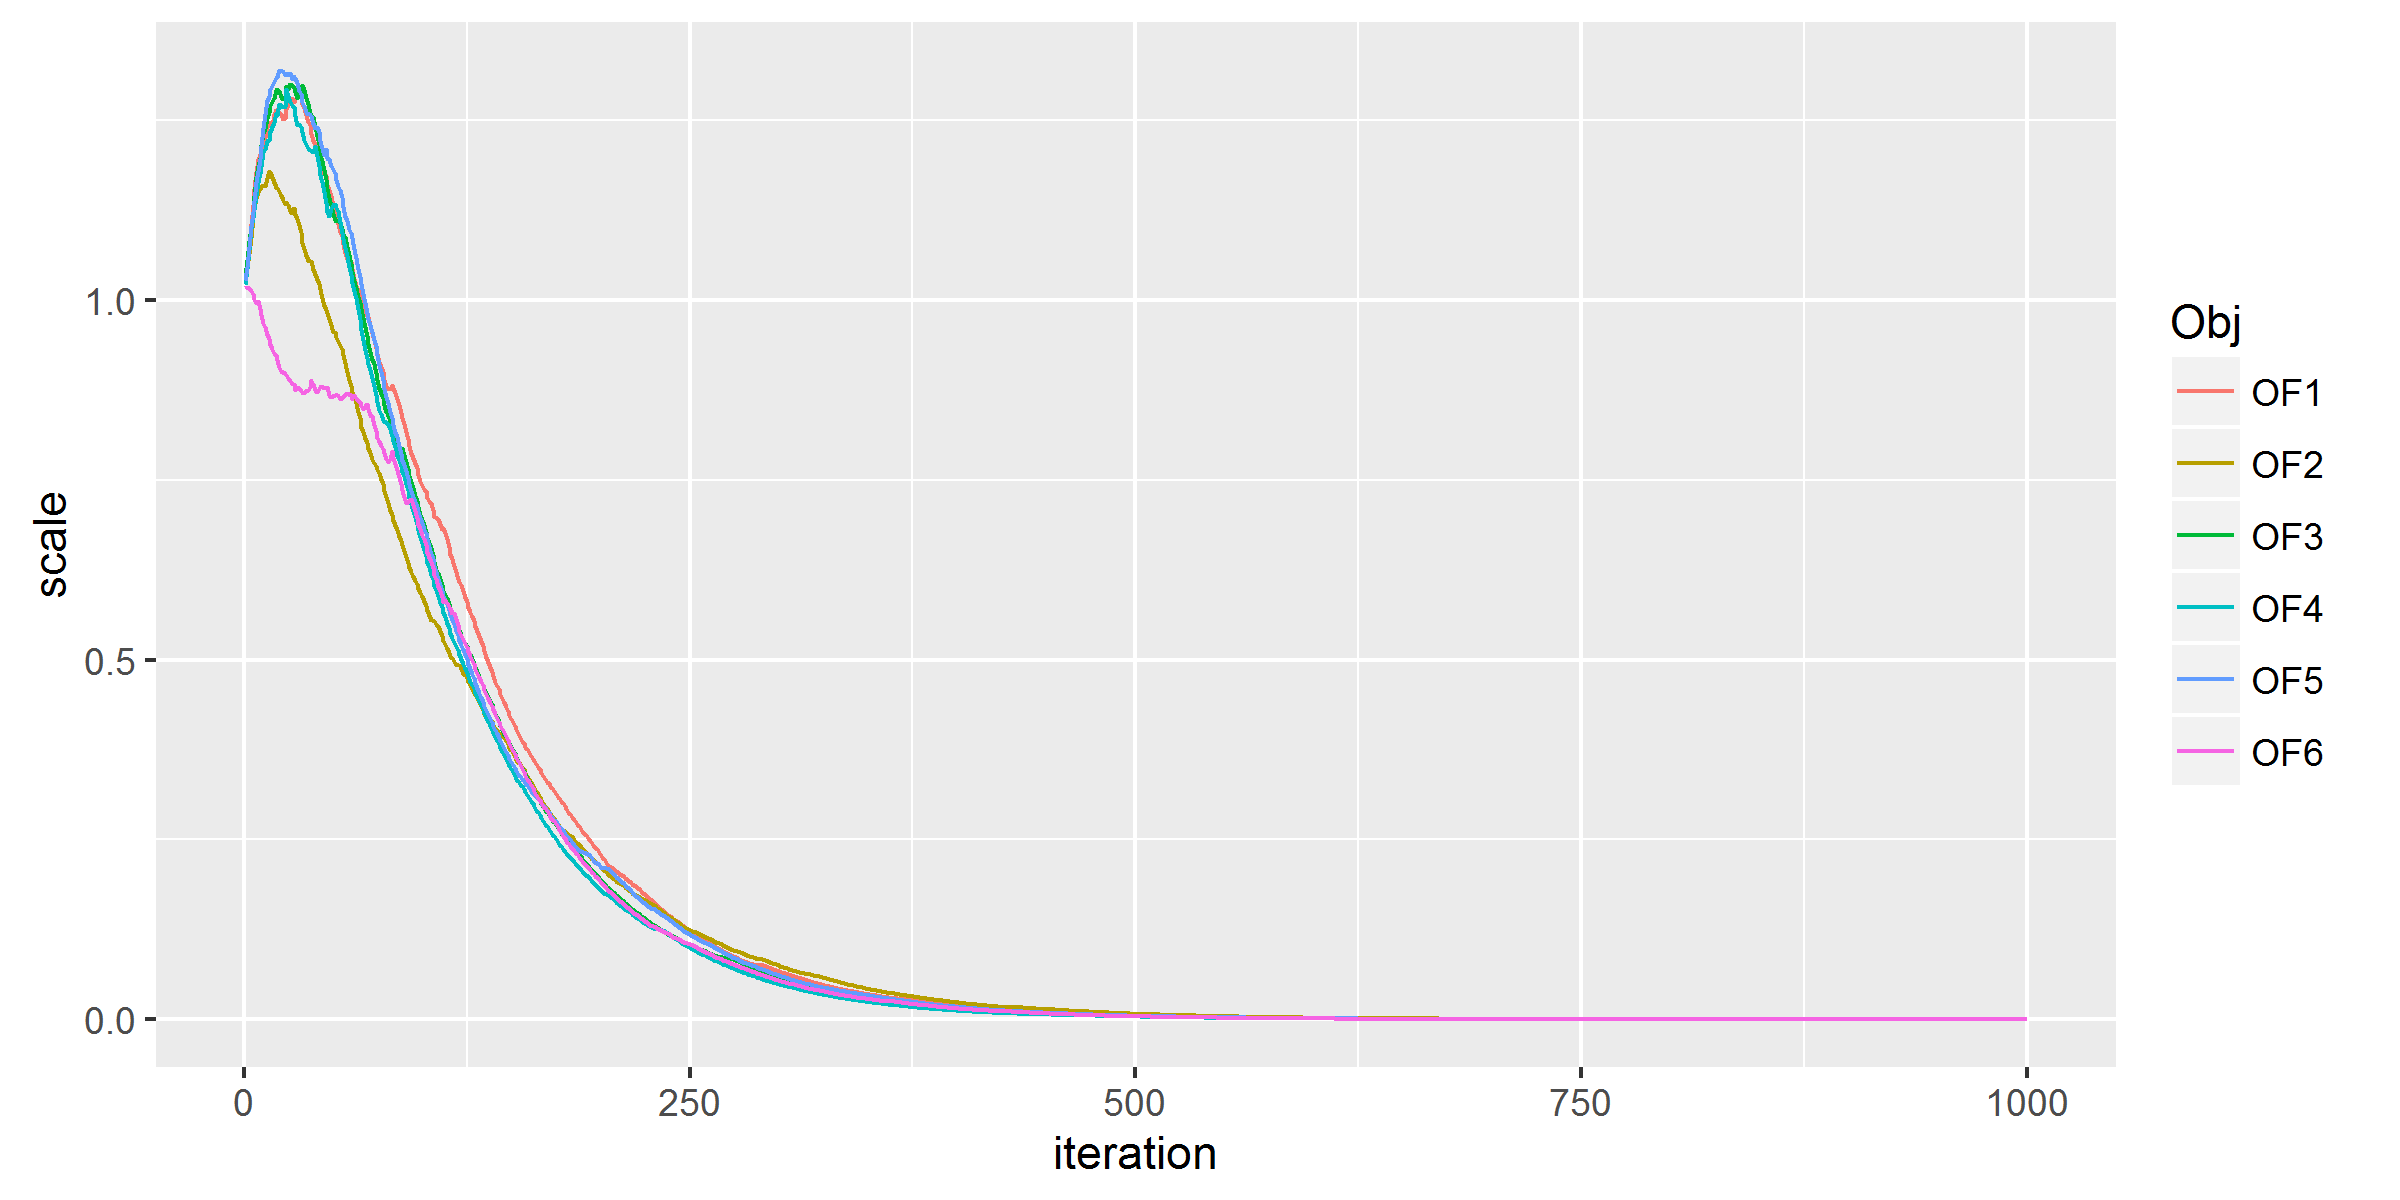
\includegraphics[width = 0.5\textwidth]{../doc/scaleplot.png}
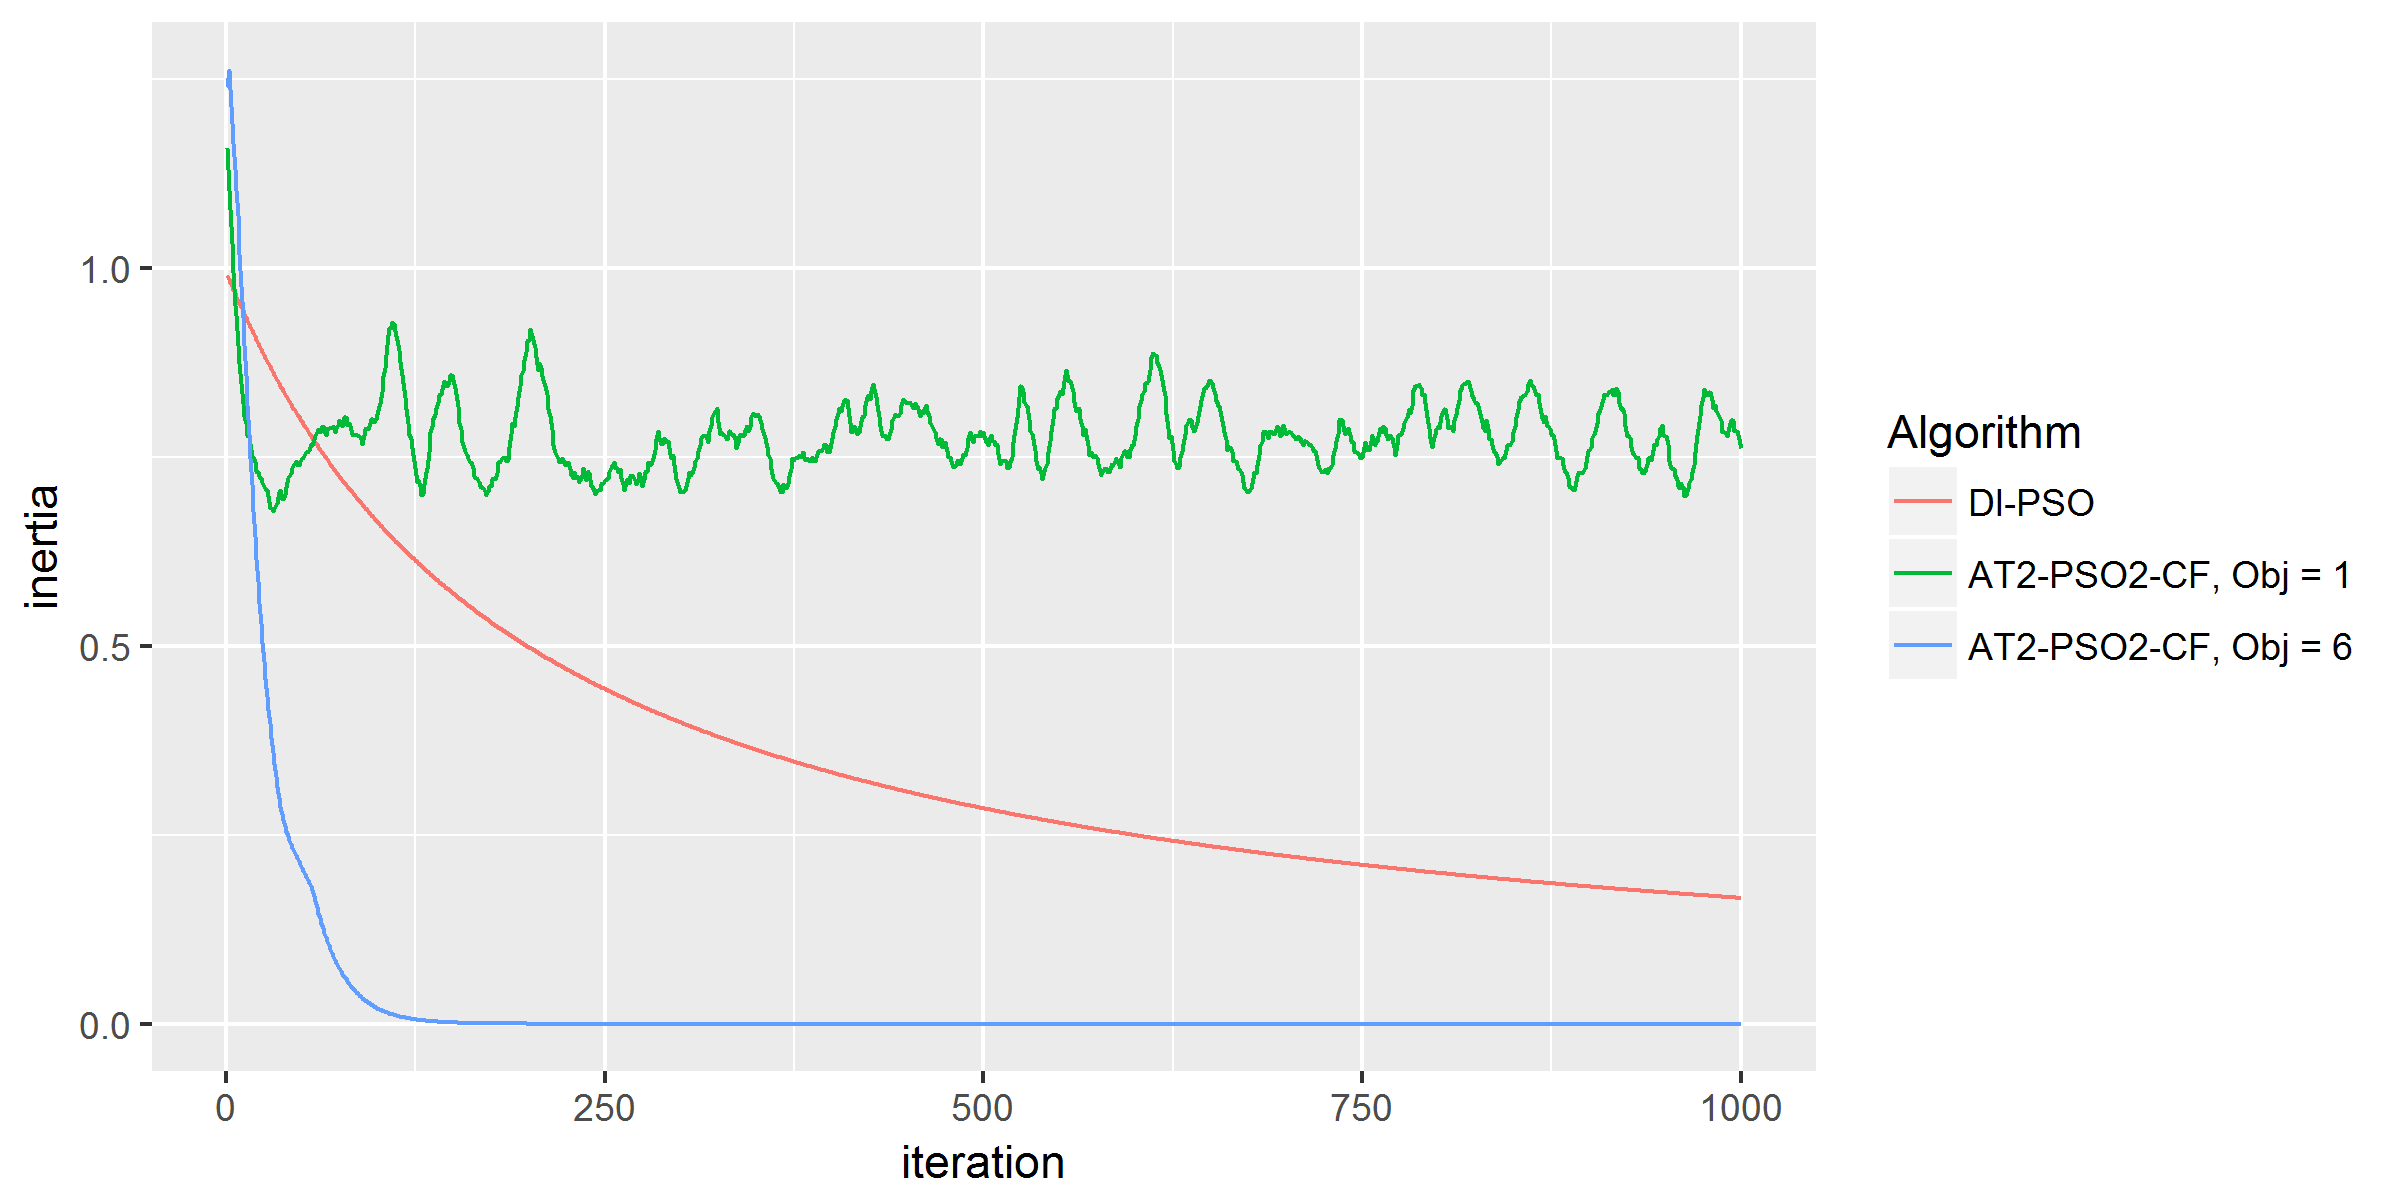
\includegraphics[width = 0.5\textwidth]{../doc/inertiaplot.png}
\pause
\begin{itemize}
\item  AT-BBPSO's scale progressions are all remarkably similar.\pause
\item  Often AT-BBPSO initially increases $\sigma^2(k)$ above 1, then starts decaying it to zero --- initial burst of high-exploration... sometimes.\pause
\item  DI-PSO's inertia has a nice smooth progression towards zero. \pause
\item  AT-PSO's inertia typically bounces around a flat trendline.\\
$\to$ Alternating between \emph{relative} exploration and exploitation. \pause
\item  AT-PSO's inertia crashes to zero when it converges. \\
$\to$ May be premature local convergence.
\end{itemize}
\end{frame}

\begin{frame}
\frametitle{Comparing AT-PSO/BBPSO to PSO/BBPSO}
Tuning $\omega(k)/\sigma^2(k)$ allows the swarm to adjust the exploration / exploitation tradeoff based on local conditions.
\begin{itemize}
\item This has a tendency to speed up convergence.
\item ...but convergence may be premature in multi-modal problems.\\~\\
\end{itemize}

\pause

Overview of results from a simulation study with a variety of objective functions:
\begin{itemize}
\item BBPSO tends to perform poorly, but AT-BBPSO performs quite well.\\
\item AT-BBPSO often the best for complex objective functions.\\
$\to$ The $\mathrm{T}_{df}$ makes it fairly robust to many local optima.\pause 
\item AT-PSO performs better than PSO on ``hard enough'' problems... \pause
\item ...but has trouble with many local optima.
\end{itemize}
\end{frame}

\begin{frame}
\frametitle{Spatial Design --- Problem Setup}
Goal: want to learn about the spatial field $Y(\bm{u})$, $\bm{u}\in\mathcal{D}\subset \mathbb{R}^2$. \pause\\~\\

We observe a noisy signal of $Y(\bm{u})$ at $N_s$ fixed monitoring locations, $\bm{s}_1, \dots, \bm{s}_{N_s}$, 
and assume:
\begin{align*}
Z(\bm{u}) = Y(\bm{u}) + \varepsilon(\bm{u})
\end{align*}
for all $\bm{u}\in\mathcal{D}$, and $\varepsilon(\bm{u}) \stackrel{iid}{\sim} \mathrm{N}(0, \tau^2)$. \pause\\~\\

Assume 
\begin{align*}
Y(\bm{u}) \sim \mathrm{GP}(\bm{x}(\bm{u})'\bm{\beta}, C(\cdot, \cdot))
\end{align*}
where $\bm{x}(\bm{u})$ is a vector of covariates known at all locations $\bm{u}\in\mathcal{D}$. \pause \\~\\

Where should we put an additional $N_d$ monitoring locations, $\bm{d}_1, \dots, \bm{d}_{N_d}$? \pause \\~\\

What if $\tau^2$, $\bm{\beta}$, and $C(\cdot, \cdot)$ are unknown?
\end{frame}

\begin{frame}
\frametitle{Spatial Design --- MSPE and Kriging}
Sensible goal: minimize MSPE in some sense.\\~\\

When $\tau^2$ and $C(\cdot, \cdot)$ are known, the universal kriging predictor is:
\begin{align*}
\widehat{Y}_{uk}(\bm{u}; \bm{d}) = \bm{x}(\bm{u})'\widehat{\bm{\beta}}_{gls} + \bm{c}_Y(\bm{u})'\bm{C}_Z^{-1}(\bm{Z} - \bm{X}\widehat{\bm{\beta}}_{gls})
\end{align*}
\citep{cressie2011statistics} where
\begin{align*}
\bm{X} &= (\bm{x}(\bm{s}_1), \dots, \bm{x}(\bm{s}_{N_s}), \bm{x}(\bm{d}_1, \dots, \bm{x}(\bm{d}_{N_d}))',\\
\bm{Y} &= (Y(\bm{s}_1), \dots, Y(\bm{s}_{N_s}), Y(\bm{d}_1), \dots, Y(\bm{d}_{N_d}))',\\
\bm{Z} &= (Z(\bm{s}_1), \dots, Z(\bm{s}_{N_s}), Z(\bm{d}_1), \dots, Z(\bm{d}_{N_d}))',\\
\bm{C}_Z &= \mathrm{Cov}(\bm{Z}) = \tau^2\bm{\mathrm{I}} + \mathrm{Cov}(\bm{Y}),\\
\bm{c}_Y &= \mathrm{Cov}(Y(\bm{u}), \bm{Y}),\\
\widehat{\bm{\beta}}_{gls} &= (\bm{X}'\bm{C}_Z^{-1}\bm{X})^{-1}\bm{X}'\bm{C}_Z^{-1}\bm{Z}.
\end{align*}
\end{frame}

\begin{frame}
\frametitle{Spatial Design --- Kriging Variances}
Kriging MSPE: \ \ $\mathrm{E}\left\{Y(\bm{u}) - \widehat{Y}_{uk}(\bm{u})\right\}^2 = \sigma_{uk}^2(\bm{u};\bm{d})=$
\begin{align*}
&C(\bm{u}, \bm{u}) - \bm{c}_Y(\bm{u})'\bm{C}_Z^{-1}\bm{c}_Y(\bm{u})\\
& + \{\bm{x}(\bm{u})  - \bm{X}'\bm{C}_Z^{-1}\bm{c}_Y(\bm{u})\}'(\bm{X}'\bm{C}_Z^{-1}\bm{X})^{-1}\{\bm{x}(\bm{u})  - \bm{X}'\bm{C}_Z^{-1}\bm{c}_Y(\bm{u})\}
\end{align*}
\pause
What about when $\tau^2$ and/or $C(\cdot, \cdot)$ are estimated?\\
$\to$ Parameter uncertainty universal kriging MSPE:
\begin{align*}
\mathrm{E}\left\{Y(\bm{u}) - \widehat{Y}_{uk}(\bm{u})\right\}^2 \approx \sigma^2_{puk}(\bm{u};\bm{d},\widehat{\bm{\theta}}) = \sigma^2_{uk}(\bm{u};\bm{d},\widehat{\bm{\theta}}) + \mbox{ stuff, }
\end{align*}
depending on the Fisher information matrix and the MLE of all parameters, denoted by $\widehat{\bm{\theta}}$ \citep{zimmerman1992mean,abt1999estimating}.
\end{frame}

\begin{frame}
\frametitle{Spatial Design --- Design Criteria}
Ideal design criteria: choose design points to minimize...
\begin{itemize}
\item Mean/total MSPE: $\int_{\mathcal{D}}\sigma^2(\bm{u})d\bm{u}$
\item Maximum MSPE: $\max_{\bm{u}\in\mathcal{D}}\sigma^2(\bm{u})$\\~\\
\end{itemize}

\pause

This is computationally infeasible. \pause \\~\\

Realistic criteria: approximate with a grid of target points $\bm{r}_1,\dots,\bm{r}_{N_t}$:
\begin{itemize}
\item Minimize $\sum_{i=1}^{N_t}\sigma^2(\bm{r}_i)$ 
\item Minimize $\max_{i=1,2,\dots,N_t}\sigma^2(\bm{r}_i)$
\end{itemize}
\end{frame}


\appendix
\newcounter{finalframe}
\setcounter{finalframe}{\value{framenumber}}

\begin{frame}

      \begin{center}

        \font\endfont = cmss10 at 25.40mm
        \color{MUgold}
        \endfont 
        \baselineskip 20.0mm

        Thank you!

      \end{center}    


\end{frame}

\begin{frame}[allowframebreaks]
        \frametitle{References}
        \bibliographystyle{apalike}
        \bibliography{../doc/pso}
\end{frame} 
\setcounter{framenumber}{\value{finalframe}}
\end{document}
